%\documentclass[12pt]{article}    % <--- 12pt font
%\usepackage[margin=1in]{geometry}% <--- 1 in margin
                  % <--- double space
\documentclass[12pt]{amsart}
\usepackage[utf8]{inputenc}
\usepackage[a4paper,margin=1in,footskip=0.25in]{geometry}
\usepackage{setspace}
\doublespace    
% See geometry.pdf to learn the layout options. There are lots.
\geometry{letterpaper}                   % ... or a4paper or a5paper or ... 
%\geometry{landscape}                % Activate for for rotated page geometry
%\usepackage[parfill]{parskip}    % Activate to begin paragraphs with an empty line rather than an indent
\usepackage{float}
\usepackage{graphicx}
\usepackage{amssymb}
\usepackage{epstopdf}
\usepackage{amsmath}
\newtheorem{thm}{Theorem}
%\usepackage{algorithm}
\usepackage{subfig}
\usepackage[authoryear]{natbib}
%\usepackage{subcaption}
\usepackage[ruled,vlined]{algorithm2e}
%\linespread{1.5}
\usepackage{comment}
\usepackage{booktabs}
\usepackage{listings}
\usepackage{color}

\definecolor{dkgreen}{rgb}{0,0.6,0}
\definecolor{gray}{rgb}{0.5,0.5,0.5}
\definecolor{mauve}{rgb}{0.58,0,0.82}

\lstset{frame=tb,
  language=python,
  aboveskip=3mm,
  belowskip=3mm,
  showstringspaces=false,
  columns=flexible,
  basicstyle={\small\ttfamily},
  numbers=none,
  numberstyle=\tiny\color{gray},
  keywordstyle=\color{blue},
  commentstyle=\color{dkgreen},
  stringstyle=\color{mauve},
  breaklines=true,
  breakatwhitespace=true,
  tabsize=3
}


\usepackage[colorlinks=true,linkcolor=blue, allcolors=blue]{hyperref}%

\title{STAT 517 Project}
\author{Chris Chen, Yueqi Xu}
\date{March 2022}

\begin{document}

\maketitle

\section{Introduction}
The paper we chose is \emph{A Spatial Analysis of Multivariate Output From Regional Climate Models (\cite{paper})}. The research problem of this paper is to study climate and conquer the challenge of characterization of distribution of the model output of climate model. 

Before talking about the the methods and results, we would like to first talk about the context and settings. Climate is often considered the long-term distribution of weather in a particular area. Two of the most important factors to climate are temperature and precipitation, which were used as metrics in \cite{paper}. 

Climate model is the key object of study in \cite{paper}. It attempts to represent the climate system, which consists of different components including atmosphere, oceans, sea ice, etc., while taking the impacts of human intervention into account.

While Climate models are deterministic, they have complex outputs, with uncertainties from a number of sources, including initial climate states, assumptions about forcings, understanding of physical processes, and representation of those processes in computer models.

In order to capture the range of variation in the model output, there is an increasing use of ensembles consisting to multiple model runs. These experiments may involve varying initial conditions (simple ensembles), model physics (perturbed-physics ensembles), specific models (multi-model ensembles), or some combinations of them.

However, due to constraints on factors such as models available, computation, and funding, the number of ensemble members is typically limited. Hence, the authors aimed to use statistical methods to quantify the distribution and breadth of variation of the model output in the ensemble. In order the accomplish the goal, the authors introduce a hierarchical statistical model to capture the multivariate spatial distribution of the output fields (e.g., the joint spatial distribution of temperature and precipitation) from a regional-climate-model ensemble.

\subsection{Regional Climate Models}

Atmosphere–ocean general circulation models (GCMs) couple an atmospheric model with an ocean model and seek to simulate the Earth’s global climate system. These models typically have grid boxes on the spatial scale of 200 to 500 km, which makes them great for investigating large-scale forcing that affects the global climate, but not that useful for regional and local projections.

The climate of a region is determined by processes that exist at planetary, regional, and local spatial scales and across a wide range of temporal scales (multi-decadal to sub-daily). Under the need of generating information at smaller scales based on GCM, downscaling methodologies are developed. There are two main types of downscaling, dynamical and statistical. 

Statistical downscaling uses empirical relationships to connect the GCM output to regional and local variables. This approach is computational effective, and it needs fine-scale and long-time-duration observational data, and there is some uncertainty about the stability of these empirical relationships over long periods of time, especially with varying forcings. Dynamical downscaling involves using high-resolution climate models and direct observations. 

Regional climate models (RCMs), which are the focus of the article, are based on the dynamic approach. These models typically have grid boxes on the scale of 20 to 100 km. Since they use initial conditions and time-dependent lateral boundary conditions from the GCM, the global circulation and large-scale forcings are consistent with the GCM. The resolution forcing in RCM is higher than that in GCM. Hence RCMs can be influenced by potential biases in the GCM, but the effect is only one-way.

\subsection{A statistical representation of climate-model output}

The statistical model for combining the output from ensembles of RCMs is formulated through the three-level hierarchical formulation, including data model, process model, and parameter model (prior distribution). \cite{paper} is the first approach of this kind for a spatial analysis of multivariate output from RCMs.

At the heart of this statistical model is an implementation of a multivariate Markov random field (MRF). MRF models are excellent tools for analyzing data laid out on regular spatial lattices. Gaussian MRF models represent the conditional expectation of an observation at a spatial location as a linear combination of observations at neighboring locations. In addition, using a MRF formulation will allow us to incorporate computational advantages (recall Lab 3). Furthermore, the multivariate nature of the statistical model will allow for more complex inferences.

\section{MRF and CAR models}

The basic framework of MRF model is, for random variables $y_1 , \dots, y_n$ observed at $n$ locations on a spatial-lattice structure, the collection of conditional distributions $f(y_i |y_{-i}), \, i = 1, \dots, n$ can be combined under certain regularity conditions to form a joint distribution $f (y_1, \dots, y_n)$.

\subsection{Univariate CAR Models}

Assuming Gaussian conditional distributions for $f (y_i |y_{-i})$, the conditional mean and conditional variance associated with $f (y_i |y_{-i})$ are specified as
$$E[y_i | y_{-i}] = \mu_i + \sum_{j\neq i}^n b_{ij} (y_j-\mu_j) \quad \text{and} \quad Var[y_i |y_{-i}] = \tau^2 > 0,$$
where $b_{ii} = 0; \, i = 1, \dots, n$. Under regularity conditions, this collection of conditional distributions gives rise to a joint Gaussian distribution,
$$N(\boldsymbol{\mu}, (\boldsymbol{I}-\boldsymbol{B})^{-1}\boldsymbol{T},$$
where $\mu=(\mu_1,\dots,\mu_n)'$, $\boldsymbol{I}$ is an $n\times n$ identity matrix, $\boldsymbol{B}$ is the $n\times n$ matrix with the $(i, j )$-th element $b_{ij}$ , and $\boldsymbol{T} = diag(\tau_{12}, \dots, \tau_{n2})$. $(\boldsymbol{I}-\boldsymbol{B})^{-1}\boldsymbol{T}$ is symmetric and positive-definite.

\subsection{Multivariate CAR models}

In the multivariate setting, there is more than one measurement at each lattice point. In particular, let $y_i$ be a p-dimensional random vector. Then, for $i = 1, \dots, n$,
$$E[\boldsymbol{y}_i | \boldsymbol{y}_{-i}] = \boldsymbol{\mu}_i + \sum_{j\neq i} \boldsymbol{B}_{ij} (\boldsymbol{y}_j-\boldsymbol{\mu}_j) \quad \text{and} \quad Var[\boldsymbol{y}_i |\boldsymbol{y}_{-i}] = \boldsymbol{T}_i,$$
where $\boldsymbol{\mu}_i$ is a p-dimensional vector, $\boldsymbol{B}_{ij}$ is a $p\times p$ matrix, and $\boldsymbol{T}_i$ is a $p\times p$ covariance matrix. 

Assume that $\boldsymbol{B}_{ij} \boldsymbol{T}_j = \boldsymbol{T}_i \boldsymbol{B}_{ji}'$ for all $i,j = 1,\dots,n$, $\boldsymbol{B}_{ii} = -\boldsymbol{I}$ and $\boldsymbol{B}_{ij} \neq 0$ for $j \in N_i$ and $i = 1,\dots,n$. Under the assumption that the $np \times np$ matrix Block($-\boldsymbol{B}_{ij}$) is positive-definite, $\boldsymbol{y} = (\boldsymbol{y}_1',\dots,y_n')'$ follows a $N(\boldsymbol{\mu}, \Sigma)$ distribution where $\boldsymbol{\mu} = (\boldsymbol{\mu}_1',\dots,\boldsymbol{\mu}_n')'$ and $ \Sigma = (Block(-\boldsymbol{T}^{-1}_i \boldsymbol{B}_{ij} ))^{-1}$.

However, the multivariate CAR models are difficult to implement in practice without dramatic simplification of the matrices representing the spatial dependence parameters [e.g., \cite{bill}] or the use of restrictive priors on the elements of these same matrices [\cite{sain2}].

\section{An alternative formulation of a multivariate MRF.}

Fundamental to this approach is thinking of multivariate lattice data as univariate data on a more complex lattice structure. In particular, this more complex lattice structure is conceptualized as a “stacking” of the lattices associated with each variable. Neighborhoods are defined by connections between locations for each variable within a lattice and again for locations across each lattice structure. A two-dimensional example of these different types of neighborhoods is shown in \ref{fig: neighborhood}.

\begin{figure}[H]
    \centering
    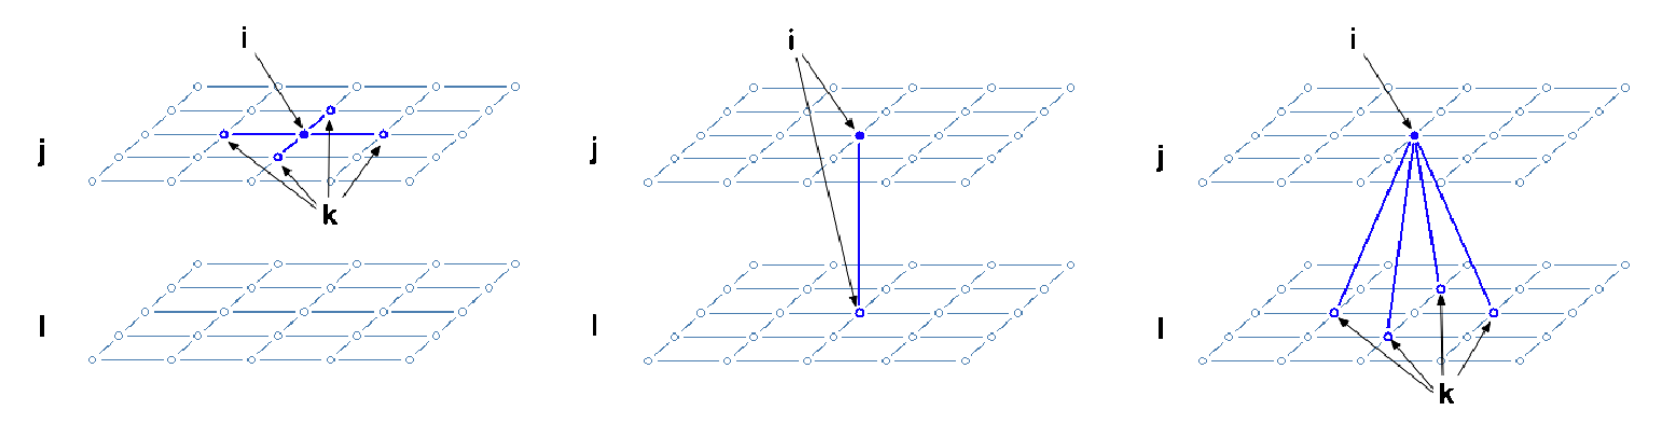
\includegraphics[width = 0.8\textwidth]{neighborhoods.png}
    \caption{Examples of different types of neighborhoods. The left frame shows a within-variable spatial neighborhood, while the middle frame shows a within-location neighborhood. The right frame demonstrates the neighborhood associated with cross-variable connections.}
    \label{fig: neighborhoods}
\end{figure}

The key feature of this approach is that it still falls within the original univariate framework of \cite{besag} outlined in Section 2.1 with
$$E[y_{ij} | y_{-ij}] = \mu_{ij} + \sum_{k \neq i} b_{ijkj} (y_{kj}-\mu_{kj}) +  \sum_{\ell \neq j} b_{iji\ell} (y_{i \ell}-\mu_{i \ell}) + \sum_{k,\ell \neq i,j} b_{ijk\ell} (y_{k\ell}-\mu_{k\ell})$$
and
$$Var[y_{ij} | y_{-ij}] = \tau_{ij}^2,$$
for all lattice points $i = 1, \dots,n$ and variables $j = 1, \dots,p$. In the conditional mean, the coefficients in the first summation represent connections within a particular layer and control conditional dependence between the $i$th lattice point and neighboring points for the $j$th variable (left frame in \ref{fig: neighborhood}). The coefficients in the
second summation represent connections across layers at the same lattice point and control conditional dependence between variables $j$ and $\ell$ at the $i$th lattice point (middle frame in \ref{fig: neighborhood}). Finally, the coefficients in the third summation represent connections between locations across layers for different variables and control conditional cross-spatial dependence (right frame in \ref{fig: neighborhood}). 

Now we see that the joint distribution is Gaussian with mean given by $\boldsymbol{\mu} = [\boldsymbol{\mu}_1' , \dots, \boldsymbol{\mu}_n']'$ and $\boldsymbol{\mu}_i = [\mu_{i1}, \dots, \mu_{ip}]'$, and with an $np \times np$ covariance matrix given by
\begin{eqnarray*}
    \begin{bmatrix}
        \boldsymbol{A}_1 & \boldsymbol{B}_{12} \delta_{12} & \cdots & & \boldsymbol{B}_{1n}\delta_{1n} \\
        \boldsymbol{B}_{21}\delta_{21} & \boldsymbol{A}_2 & & & \vdots \\
        \vdots & & \ddots &  & \\
        & & & \boldsymbol{A}_{n-1} & \boldsymbol{B}_{n-1, n}\delta_{n-1, n} \\
        \boldsymbol{B}_{n1}\delta_{n1} & \cdots &  & \boldsymbol{B}_{n, n-1}\delta_{n, n-1} &  \boldsymbol{A}_n
    \end{bmatrix}^{-1} \boldsymbol{T},
\end{eqnarray*}
where $\delta_{ik} =1$ if $k \in N_i$ and 0 otherwise. Each $p\times p$ block is given by
$$
    \boldsymbol{A}_i = \begin{bmatrix}
        1 &  & -b_{ijk\ell} \\
         & \ddots  &  \\
        -b_{i\ell ij} &  & 1 
    \end{bmatrix} \quad \text{or} \quad
    \boldsymbol{B}_{ik} = \begin{bmatrix}
        -b_{i1k1} &  & -b_{ijk\ell} \\
         & \ddots  &  \\
        -b_{i\ell kj} &  & -b_{ipkp}
    \end{bmatrix},
$$
where $-b_{iji\ell}$ and $-b_{i\ell ij}$ are arbitrary off-diagonal elements of $\boldsymbol{A}_i$, and $-b_{ijk\ell}$ and $-b_{i\ell kj}$ are arbitrary off-diagonal elements of $\boldsymbol{B}_{ik}$. Finally, $\boldsymbol{T} = \text{diag}(\tau_{11}^2, \dots, \tau_{1p}^2, \dots, \tau_{n1}^2, \dots, \tau_{np}^2)$. 

\section{A hierarchical model for an RCM experiment}

Let the n-dimensional vector $\boldsymbol{y}_{rj}$ denote the output of an RCM, in particular, the $r$th ensemble member for the $j$th variable. \cite{paper} focused solely on simple ensembles; that is, each member of the ensemble represents a perturbation of initial conditions for a single model.

At the first level of the hierarchy, the data model assumes that the vectors $\boldsymbol{y}_{rj}, \, r =1, \dots,m,j =1, \dots,p$, are independent with
$$\boldsymbol{y}_{rj} | \boldsymbol{\alpha}_j, \, \boldsymbol{\beta}_{rj}, \boldsymbol{h}_{rj}, \sigma^2_j \sim N(\boldsymbol{X}_1 \boldsymbol{\alpha}_j + \boldsymbol{X}_2 \boldsymbol{\beta}_{rj} + \boldsymbol{h}_{rj}, \, \sigma_j \boldsymbol{I}),$$
where $m$ indicates the number of ensemble members. $\boldsymbol{X}_1 \boldsymbol{\alpha}_j$ is the fixed effects common to all ensemble members within the $j$th variable, $\boldsymbol{X}_2 \boldsymbol{\beta}_{rj}$ is the random effects specific to the $r$th ensemble member within the $j$th variable, $\boldsymbol{h}_{rj}$ includes the Spatial random effects, and $\sigma_j$ represents a variable-specific variance.

The process model has two parts. First, the vectors $[\boldsymbol{\beta}_{r1}',\dots,\boldsymbol{\beta}_{rp}']', \, r = 1, \dots, m$, are assumed to be independent with
$$  \left .
    \begin{pmatrix}
        \boldsymbol{\beta}_{r1} \\
        \vdots \\
        \boldsymbol{\beta}_{rp}
    \end{pmatrix}  \right \vert
    \begin{pmatrix}
        \boldsymbol{\beta}_{1} \\
        \vdots \\
        \boldsymbol{\beta}_{p}
    \end{pmatrix}, \quad \boldsymbol{\Sigma}_b \sim N \left(   
        \begin{pmatrix}
            \boldsymbol{\beta}_{1} \\
            \vdots \\
            \boldsymbol{\beta}_{p}
        \end{pmatrix}, \boldsymbol{\Sigma}_b
    \right),
$$
where $\boldsymbol{\Sigma}_b$ is a $pq \times pq$ covariance matrix with $q$ the number of columns of $\boldsymbol{X}_2$. It focuses on linking the random regression coefficients specific to each ensemble member. Second, the vectors $[\boldsymbol{h}_{r1}', \dots, \boldsymbol{h}_{rp}']', r = 1, \dots, m$, are assumed to be independent with 
$$
    \left .
    \begin{pmatrix}
        \boldsymbol{h}_{r1} \\
        \vdots \\
        \boldsymbol{h}_{rp}
    \end{pmatrix}  \right \vert
    \begin{pmatrix}
        \boldsymbol{h}_{1} \\
        \vdots \\
        \boldsymbol{h}_{p}
    \end{pmatrix}, \quad \{\tau_j^2\}, \{\rho_{j\ell}\}, \{\phi_{j\ell}\} \sim N \left(   
        \begin{pmatrix}
            \boldsymbol{h}_{1} \\
            \vdots \\
            \boldsymbol{h}_{p}
        \end{pmatrix}, \boldsymbol{V}(\{\tau_j^2\}, \{\rho_{j\ell}\}, \{\phi_{j\ell}\})
    \right).
$$
It imposes a multivariate structure on the spatial random effects. Note that the vectors $[\boldsymbol{\beta}_{r1}', \dots,\boldsymbol{\beta}_{rp}']'$ and $[\boldsymbol{h}_{r1}', \dots,\boldsymbol{h}_{rp}']'$ are assumed to be independent as well.

The final level of the hierarchy is the parameter model, which assumes prior distributions on $\{\sigma_j \}, \{\boldsymbol{\alpha}_j \}, \{\boldsymbol{\beta}_j \}, \{\boldsymbol{h}_j\}, \boldsymbol{\Sigma}_b, \{\tau_j^2\}, \{\rho_{j\ell}\}, \{\phi_{j\ell}\}$. Typically, these priors will be vague or noninformative as well as independent, and must ensure that the resulting covariance matrix is positive-definite. The posterior distribution for the three-level hierarchical model is given by
\begin{eqnarray*}
    P(\{\sigma_j \}, \{\boldsymbol{\alpha}_j \}, \{\boldsymbol{\beta}_{rj} \}, \{\boldsymbol{\beta}_{j} \} ,  \{\boldsymbol{h}_{rj}\}, \{\boldsymbol{h}_{j}\}, \boldsymbol{\Sigma}_b, \{\tau_j^2\}, \{\rho_{j\ell}\}, \{\phi_{j\ell}\}) | \boldsymbol{Y} \\
    \propto P(\boldsymbol{Y} | \{\sigma_j \}, \{\boldsymbol{\alpha}_j \}, \{\boldsymbol{\beta}_{rj} \}, \{\boldsymbol{h}_{rj}\}) \\
    \times P(\{\boldsymbol{\beta}_{rj}\} |  \{\boldsymbol{\beta}_j \}, \boldsymbol{\Sigma}_b) P(\{\boldsymbol{h}_{rj}\} | \{\boldsymbol{h}_j \}, \{\tau^2_j \}, \{\rho_{j\ell} \}, \{\phi_{j\ell}\}) \\
    \times P(\{\sigma_j \})P(\{\boldsymbol{\alpha}_j \})P(\{\boldsymbol{\beta}_j \}) P(\{\boldsymbol{h}_j\}) P(\boldsymbol{\Sigma}_b) P(\{\tau_j^2\}) P(\{\rho_{j\ell}\}, \{\phi_{j\ell}\}).
\end{eqnarray*}
Note that there is no closed-form solution for the posterior, so we use MCMC to sample from the posterior distribution. In particular, we implement a Gibbs sampler [\cite{german}; \cite{gelfand}; \cite{gelfand2}], incorporating Metropolis–Hastings steps [\cite{metropolis}; \cite{hastings}] where necessary.

One benefit of a MRF is that the specification involves the precision or inverse covariance matrix, and this matrix is typically sparse; that is, many of the elements of the matrix are zero, which gives great potential for computational efficiency. The sparse Cholesky decomposition is one of the most important computational devices for MRF models. The spam package [\cite{furrer}] has functionality that is well suited for implementing MCMC with a MRF model.

\section{The RCM experiment}

A long-run average of weather is one way to quantify climate, typical summaries of climate model runs include seasonal averages of temperature and precipitation with the length of the integration often determined by computational considerations. Hence, twenty-year winter (December, January, and February) average temperature and average total precipitation were computed for each grid box and for each of the control and the three future runs. Differences between the future and the control were calculated, yielding change-in-temperature and change-in-total-precipitation variables. Hence, there are $p = 2$ variables and $m = 3$ ensemble members, giving six fields to be analyzed. These spatial fields for the winter season are shown in Figure \ref{fig: Fig2}. 

\begin{figure}[H]
    \centering
    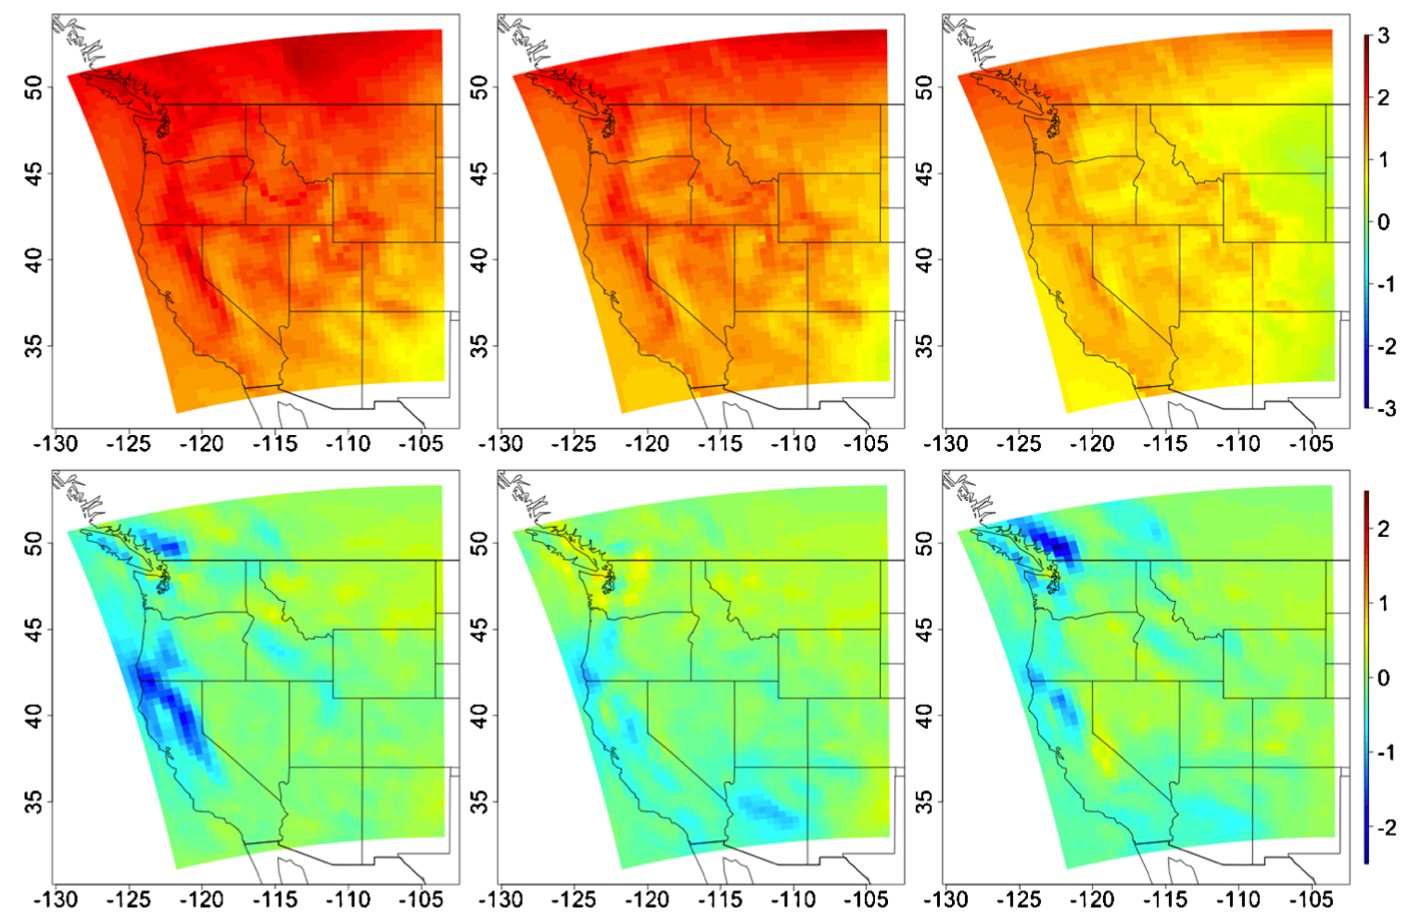
\includegraphics[width = 0.8\textwidth]{Fig2.png}
    \caption{Top row shows the three differences in winter midpoint temperature ($^\circ K$), while the bottom row shows the three differences in total precipitation (inches)}
    \label{fig: Fig2}
\end{figure}

\subsection{Model specification}

Latitude, longitude, and elevation were used as covariates in the common regression component $\boldsymbol{X}_1 \boldsymbol{\alpha}_j$, to which a random intercept across ensemble members was added $\boldsymbol{X}_2 \boldsymbol{\beta}_{rj}$. The prior covariance matrix for the random intercept was also simplified to $\Sigma_b = \sigma_b^2\boldsymbol{I}_p$.

The prior distributions are 
\begin{eqnarray*}
    P (\sigma^2 ) &\propto& 1/\sigma^2 \text{ for each } \{\sigma_j^2\} \text{ and } \sigma_b^2 \\
    \{\boldsymbol{\alpha}_i \} &\sim& N(\boldsymbol{0}, 10 \boldsymbol{I}_p) \\
    \{\boldsymbol{\beta}_j \} &\sim& N(\boldsymbol{0}, 100 \boldsymbol{I}_p) \\
    \{\boldsymbol{h}_j \} &\sim& N(\boldsymbol{0}, 10 \boldsymbol{I}_p) \\
    \{\rho \}, \{\phi_{1,1} \}, \{\phi_{1,2}\}, \{\phi_{2, 1} \}, \{\phi_{2,2} \}  &\sim& Unif(\text{range that yield a positive-definite covariance matrix})
\end{eqnarray*}
The region of uniform distribution was identified using rejection sampling based on a sparse Cholesky decomposition. Uniform priors were chosen because any concentrating priors on a subregion of the parameter space leads to a biased estimate when the true parameter lies outside this region.

\subsection{Results for the winter season.} 

Posterior distributions were obtained using MCMC algorithms. Ten chains were run, each with random starting values; the starting values for the conditional-dependence parameters were chosen uniformly across the space of values that yield a positive-definite covariance matrix.

A Gibbs sampler was implemented that involved three distinct regimes. In the first regime (2500 iterations), each of the conditional-dependence parameters was updated one at a time using a Metropolis–Hastings algorithm. Gaussian proposal distributions were used, with periodic updates of the proposal variance to achieve an approximate 20\% acceptance rate. In the second regime (the next 10,000 iterations), $\rho$, $\phi_{12}$, and $\phi_{21}$ were updated simultaneously using a Metropolis–Hastings algorithm with a multivariate Gaussian proposal distribution. Other conditional-dependence parameters were still updated using a univariate Metropolis–Hastings algorithm. Again, the proposal covariance matrix was updated periodically to achieve an approximate 20\% acceptance rate. In the third regime (the last 10,000 iterations), $\rho$, $\phi_{12}$, and $\phi_{21}$ were again updated simultaneously, but no further updates of the proposal distribution were made.

Figure \ref{fig: Fig3} shows scatterplots and kernel estimates of the distribution of $\phi_{11}$ (temperature) and $\phi_{22}$ (precipitation), the parameters that control the conditional dependence between lattice points within a layer (Figure \ref{fig: neighborhoods}, left panel). The distributions show that there is considerable (conditional) spatial dependence within each variable, with a slightly stronger dependence for temperature ($\phi_{11}$).

\begin{figure}[H]
    \centering
    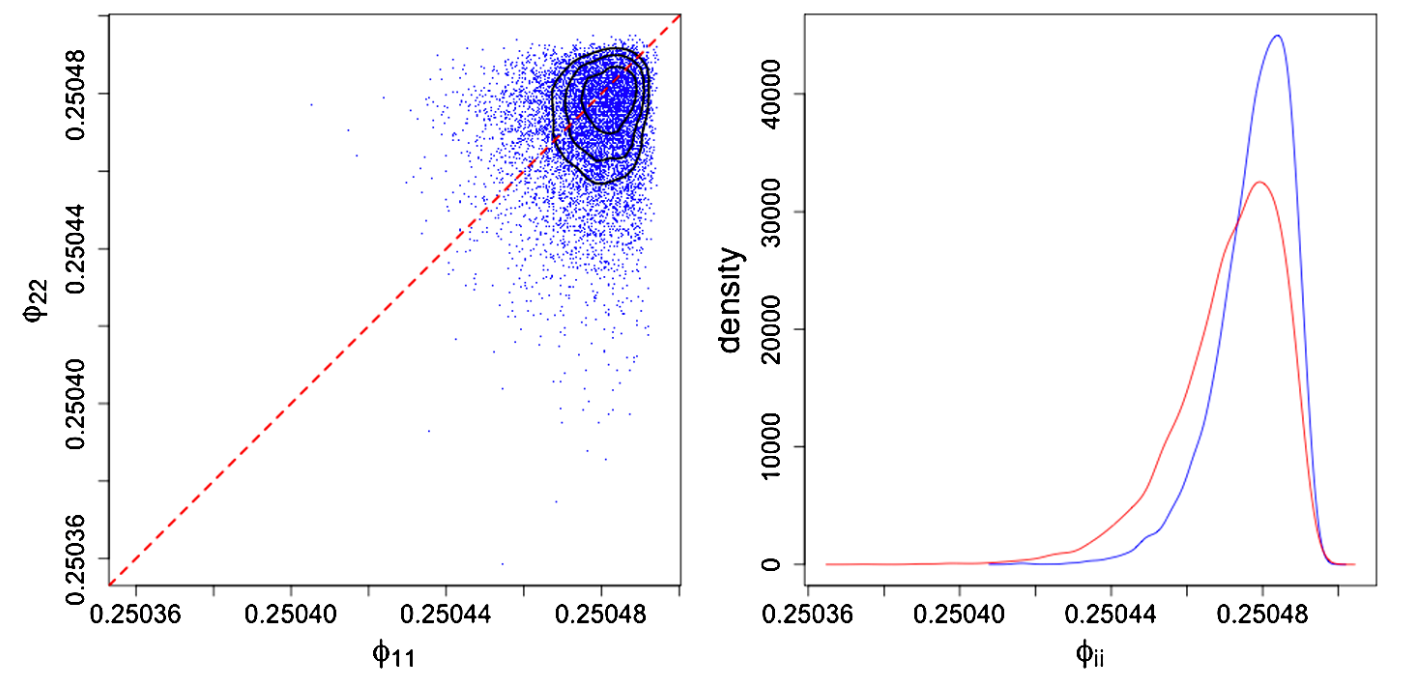
\includegraphics[width = 0.8\textwidth]{Fig3.png}
    \caption{Left frame shows scatterplot of a random sample of 10,000 values of $\phi_{11}$ and $\phi_{22}$ (1000 from each of the 10 chains). Contours represent approximate 25, 50, and 75\% contours of a kernel density estimate. Right frame shows kernel density estimates of the marginals for $\phi_{11}$ (blue) and $\phi_{22}$ (red).}
    \label{fig: Fig3}
\end{figure}

$\rho$, $\phi_{12}$, and $\phi_{21}$ control the dependence structure across variables; $\rho$ summarizes the within-location dependence (Figure \ref{fig: neighborhoods}, middle panel) and $\phi_{12}$, $\phi_{21}$ summarize the cross-variable dependence (Figure \ref{fig: neighborhoods}, right panel). The estimated posterior mean and posterior standard deviation for $\rho$ is $-0.12$ and $0.014$, respectively. A negative value for $\rho$ suggests that an increasing temperature is (conditionally) associated with a decreasing total precipitation.

Figure \ref{fig: Fig4} highlights the distribution of $\phi_{12}$ and $\phi_{21}$. These two conditional cross-correlation parameters are strongly correlated. Note that roughly 85\% of the sampled points are above the line $y = x$, which suggests that there is higher conditional dependence between temperature values and neighboring total precipitation than there is conditional dependence between total precipitation values and neighboring temperature values.

\begin{figure}[H]
    \centering
    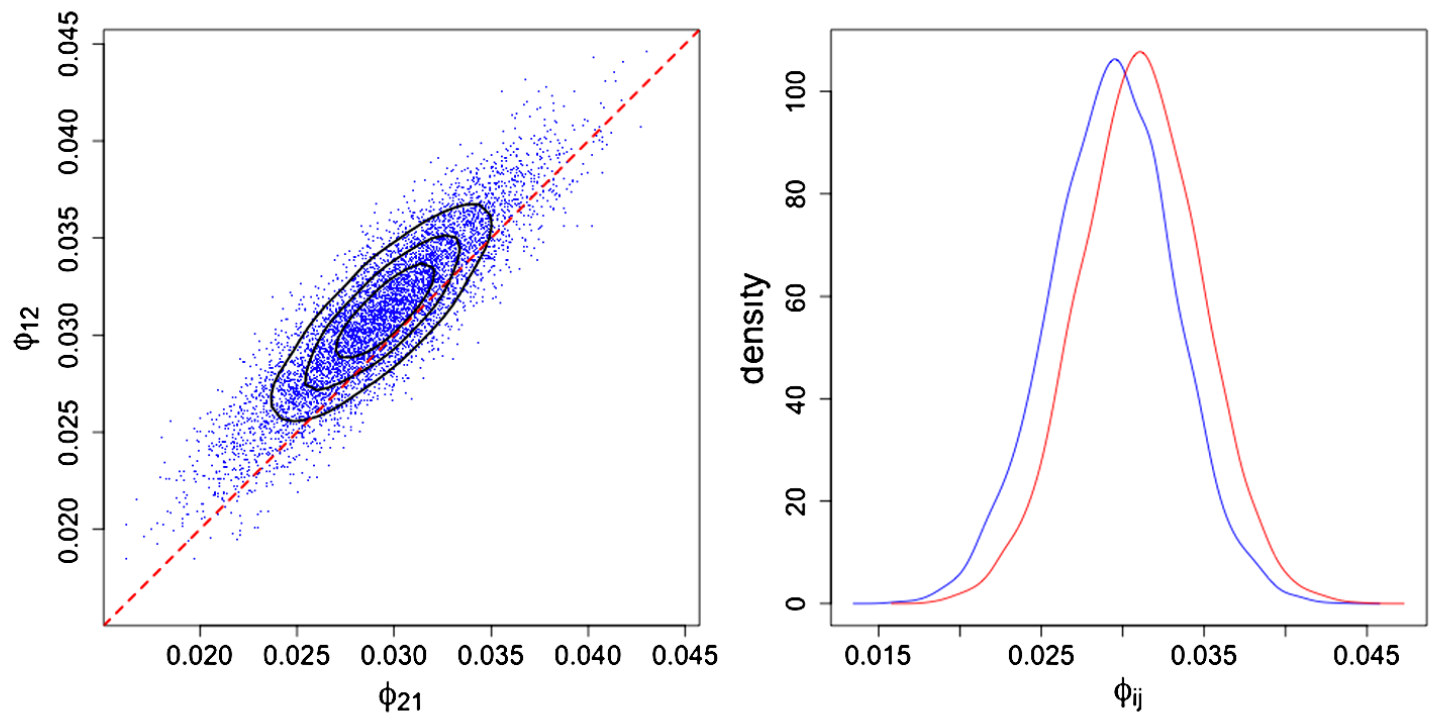
\includegraphics[width = 0.8\textwidth]{Fig4.png}
    \caption{\emph{Left frame shows scatterplot of a random sample of 10,000 values of $\phi_{12}$ and $\phi_{21}$ (1000 from each of the 10 chains). Contours represent approximate 25, 50, and 75\% contours of a kernel density estimate. Right frame shows kernel density estimates of the marginals for $\phi_{12}$ (red) and $\phi_{21}$ (blue).}}
    \label{fig: Fig4}
\end{figure}

The fixed effects in Figure \ref{fig: Fig5} show a clear latitudinal effect as well as an east-to-west gradient. For precipitation, there is a more dominant east-to-west gradient. The spatial random effects for the change in temperature seem to follow the features of the topography, and are, in general, of smaller magnitude than the fixed effects. The spatial effects for the change in total precipitation also follow the features of the topography, but there are additional strong local features, for example, in northern California. In contrast to temperature, the spatial effects for total precipitation are larger relative to the fixed effects. The sum of the fixed effects and the spatial random effects for temperature shows a consistent pattern of winter warming on average throughout the west, while the sum for total precipitation shows patterns that are much more localized. The most dominant signal for total precipitation is indicated by the regions of sharp decline in winter precipitation in northern California and the Pacific northwest.

\begin{figure}[H]
    \centering
    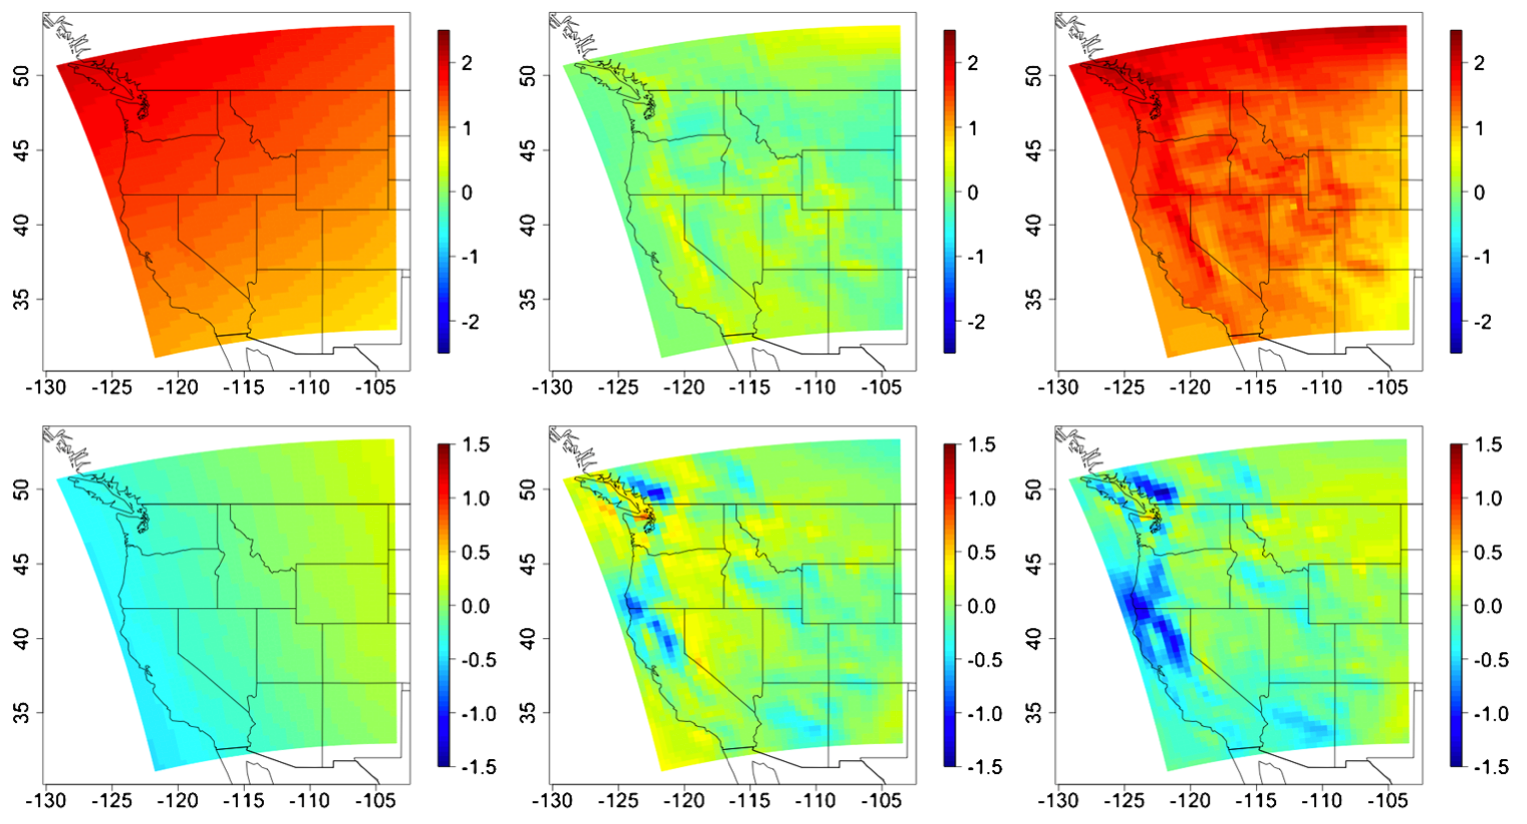
\includegraphics[width = 0.8\textwidth]{Fig5.png}
    \caption{\emph{Posterior means for the regression (left), the spatial effect (middle), and the sum (right) for the winter season. The top row represents the change in midpoint temperature ($^\circ K$), while the bottom represents the change in total precipitation (inches).}}
    \label{fig: Fig5}
\end{figure}

To aid in the identification of areas that might be at most risk for change, as projected by this regional-climate-model experiment, Figure \ref{fig: Fig6} shows the result of a hierarchical clustering based on the posterior distribution of the mean change in temperature and total precipitation for each grid. The dark red areas, for example, highlight a region associated with a strong increase in temperature and a strong decrease in total precipitation.

\begin{figure}[H]
    \centering
    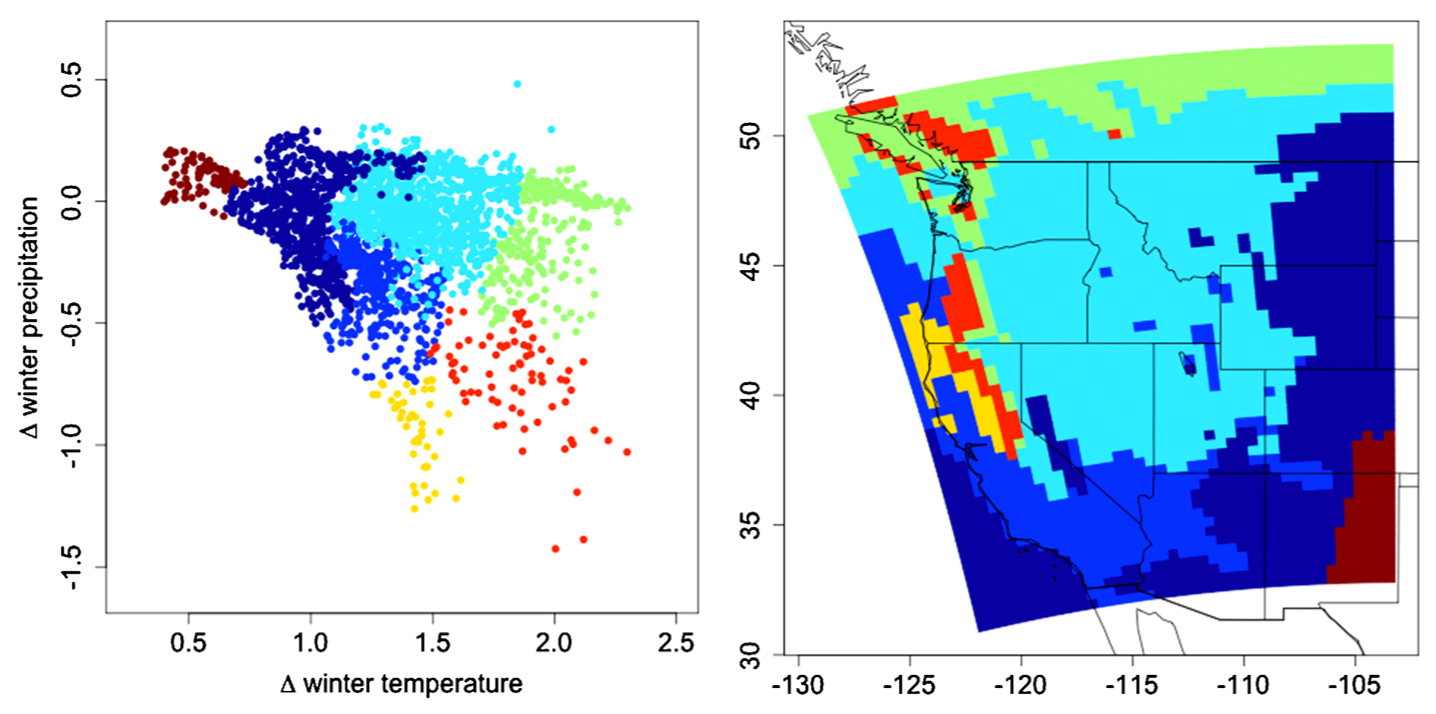
\includegraphics[width = 0.8\textwidth]{Fig6.png}
    \caption{\emph{Results from clustering the posterior means of the change in temperature and the change in total precipitation for the winter season. The left frame is a scatteplot with the clusters indicated through different colors. The right frame shows the clusters spatially.}}
    \label{fig: Fig6}
\end{figure}

Figure \ref{fig: Fig7} shows estimated pointwise probabilities based on a sampling of the posterior distribution of the joint spatial fields. In general, temperature is increasing on average across the entire domain; hence, these probabilities are based on increases larger than the median computed from all the samples across all the grid boxes. Likewise, the decrease in total precipitation was based on decreases larger than the median across all the samples from all the grid boxes. On the basis of this model, we see evidence of widespread increase in temperature and decrease in total precipitation across the western U.S.

\begin{figure}[H]
    \centering
    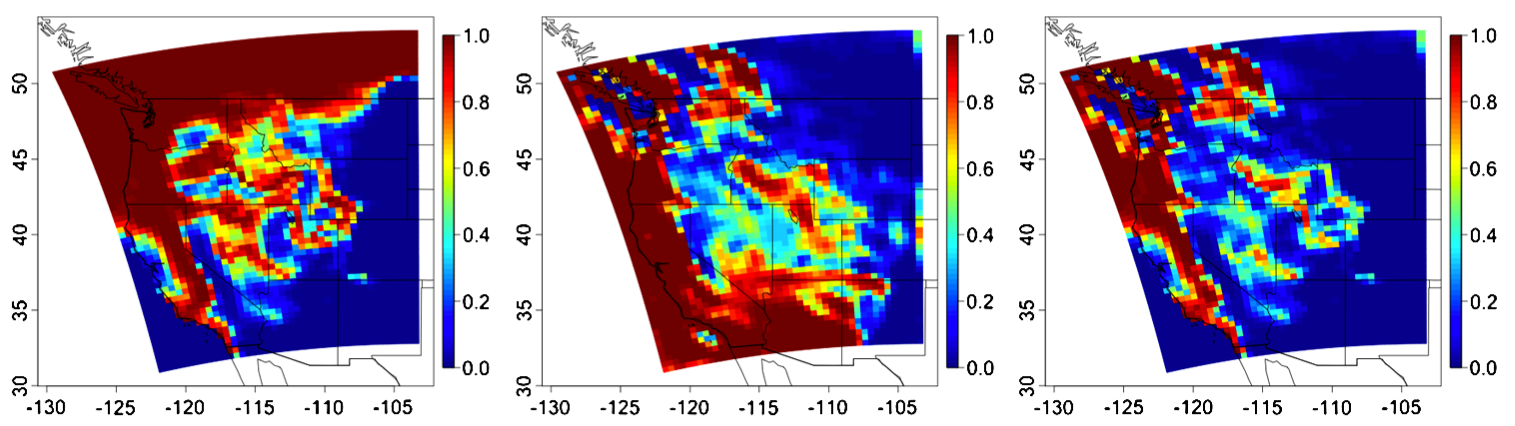
\includegraphics[width = 0.8\textwidth]{Fig7.png}
    \caption{\emph{Estimated pointwise probabilities for the winter season: increasing temperature (left), decreasing total precipitation (middle), and simultaneously increasing temperature and decreasing total precipitation (right).}}
    \label{fig: Fig7}
\end{figure}

Figure \ref{fig: Fig8} shows an alternative representation of the joint distribution by considering conditional probabilities. The figure shows the probability of the decrease in total precipitation being in the top quartile, conditional on the increase in temperature being in each of the four quartiles. As the temperature increase becomes more extreme, the largest decreases in total precipitation move from being focused in the southwest (and the California coast) to the Pacific northwest (and the California coast). 

\begin{figure}[H]
    \centering
    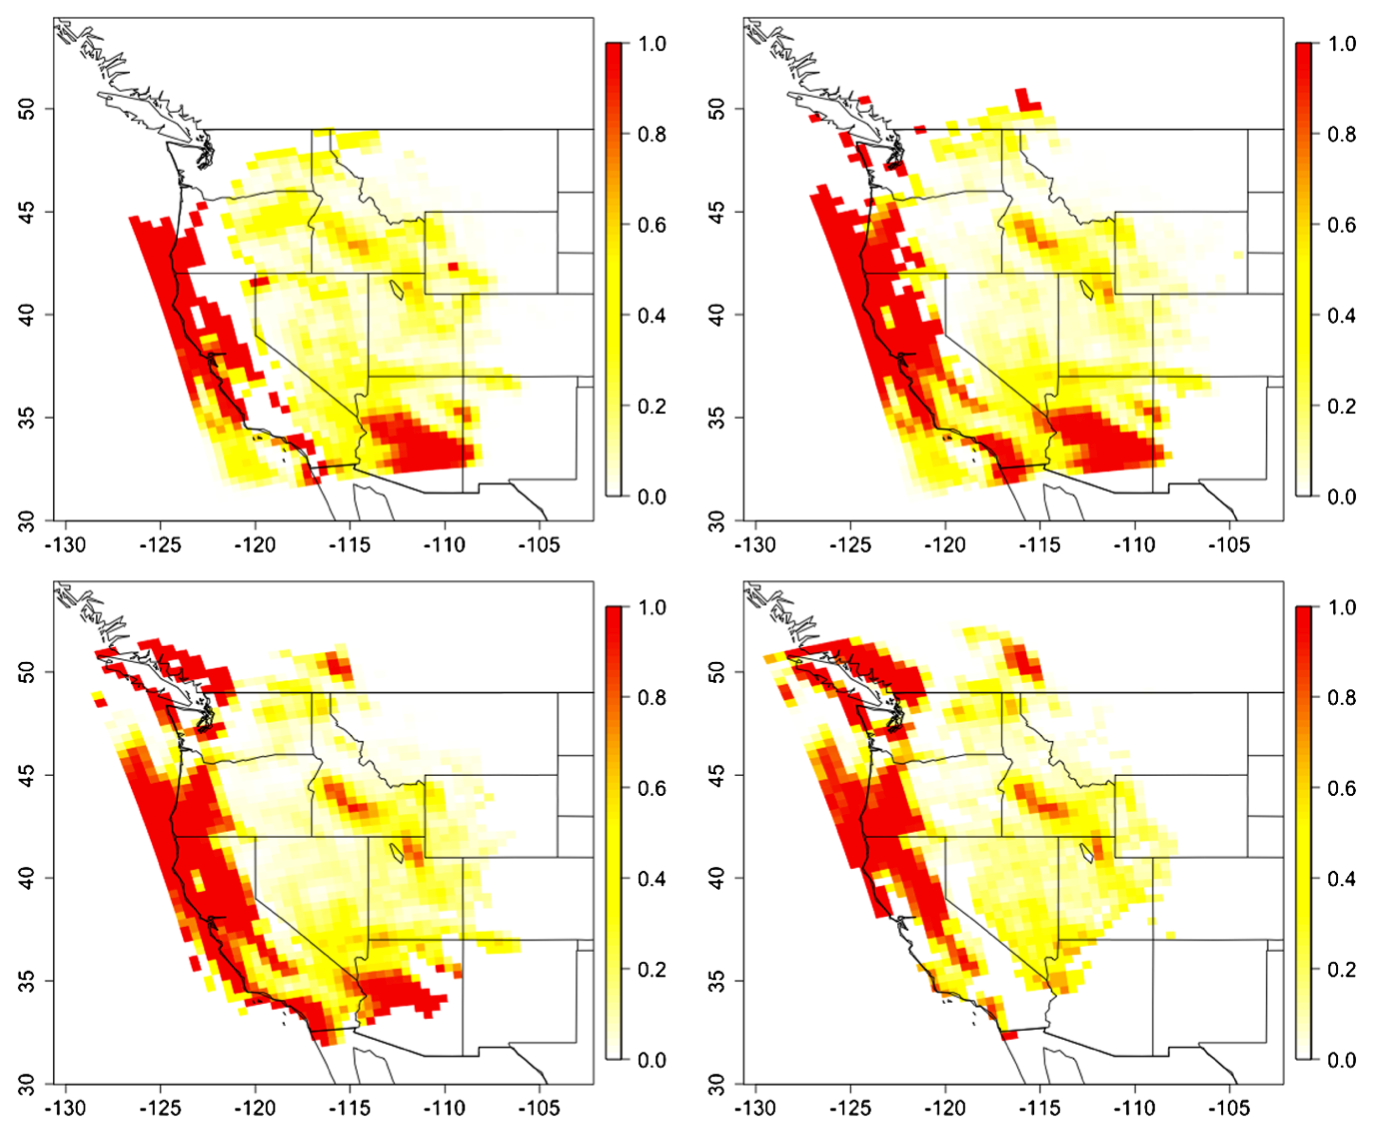
\includegraphics[width = 0.8\textwidth]{Fig8.png}
    \caption{\emph{Probability of a large decrease in winter total precipitation, conditional on the increase in temperature falling in the first quartile (top left), second quartile (top right), third quartile (bottom left), and fourth quartile (bottom right).}}
    \label{fig: Fig8}
\end{figure}

Figure \ref{fig: Fig9} suggests that the projection for the Denver area includes average increases in temperature of just under $1^\circ K$ with minimal average decreases in total precipitation. The contour for the Sacramento area, on the other hand, suggests much larger average increases in temperature and average decreases in total precipitation.

\begin{figure}[H]
    \centering
    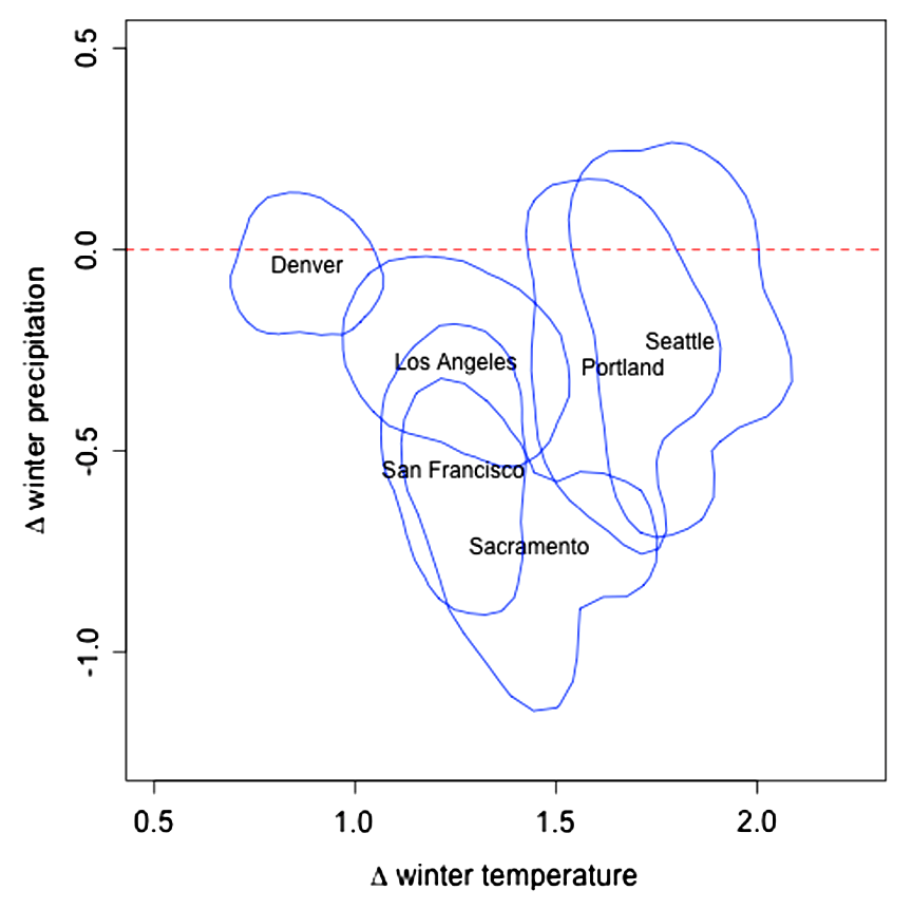
\includegraphics[width = 0.8\textwidth]{Fig9.png}
    \caption{\emph{Approximate 95\% contours for the average change in winter temperature and precipitation for the grid boxes associated with the five consolidated metropolitan statistical areas in the domain.}}
    \label{fig: Fig9}
\end{figure}

\subsection{Results for the summer season}

A slightly different scheme was used for the Gibbs sampler for the analysis of the summer model output. The three-regime sampling was still used, although with twice as many iterations (20,000) in the second regime. In addition, all five conditional-dependence parameters ($\rho, \phi_{11}, \phi_{12}, \phi_{21}. \phi_{22}$) were updated simultaneously. Posterior mean of $\rho$ is $-0.41$ for summer versus $-0.12$ for winter, suggesting that the summer season has a much stronger and more negative correlation between the change in temperature and the change in total precipitation.

Figure \ref{fig: Fig10} shows posterior means for the summer. Now there appears to be a west-to-east gradient in the fixed effects for temperature, and, again, the spatial random effects pick up more of the topography that is not accounted for in the fixed effects. Again, for temperature, the spatial random effects are of smaller magnitude than the fixed effects.

For total precipitation, there is also a west-to-east gradient in the fixed effects. The spatial random effects for the change in total precipitation also follow the features of the topography, but there are strong local features, now occurring in the eastern part of the domain. In comparison to temperature, the spatial random effects are larger relative to the fixed effects.

\begin{figure}[H]
    \centering
    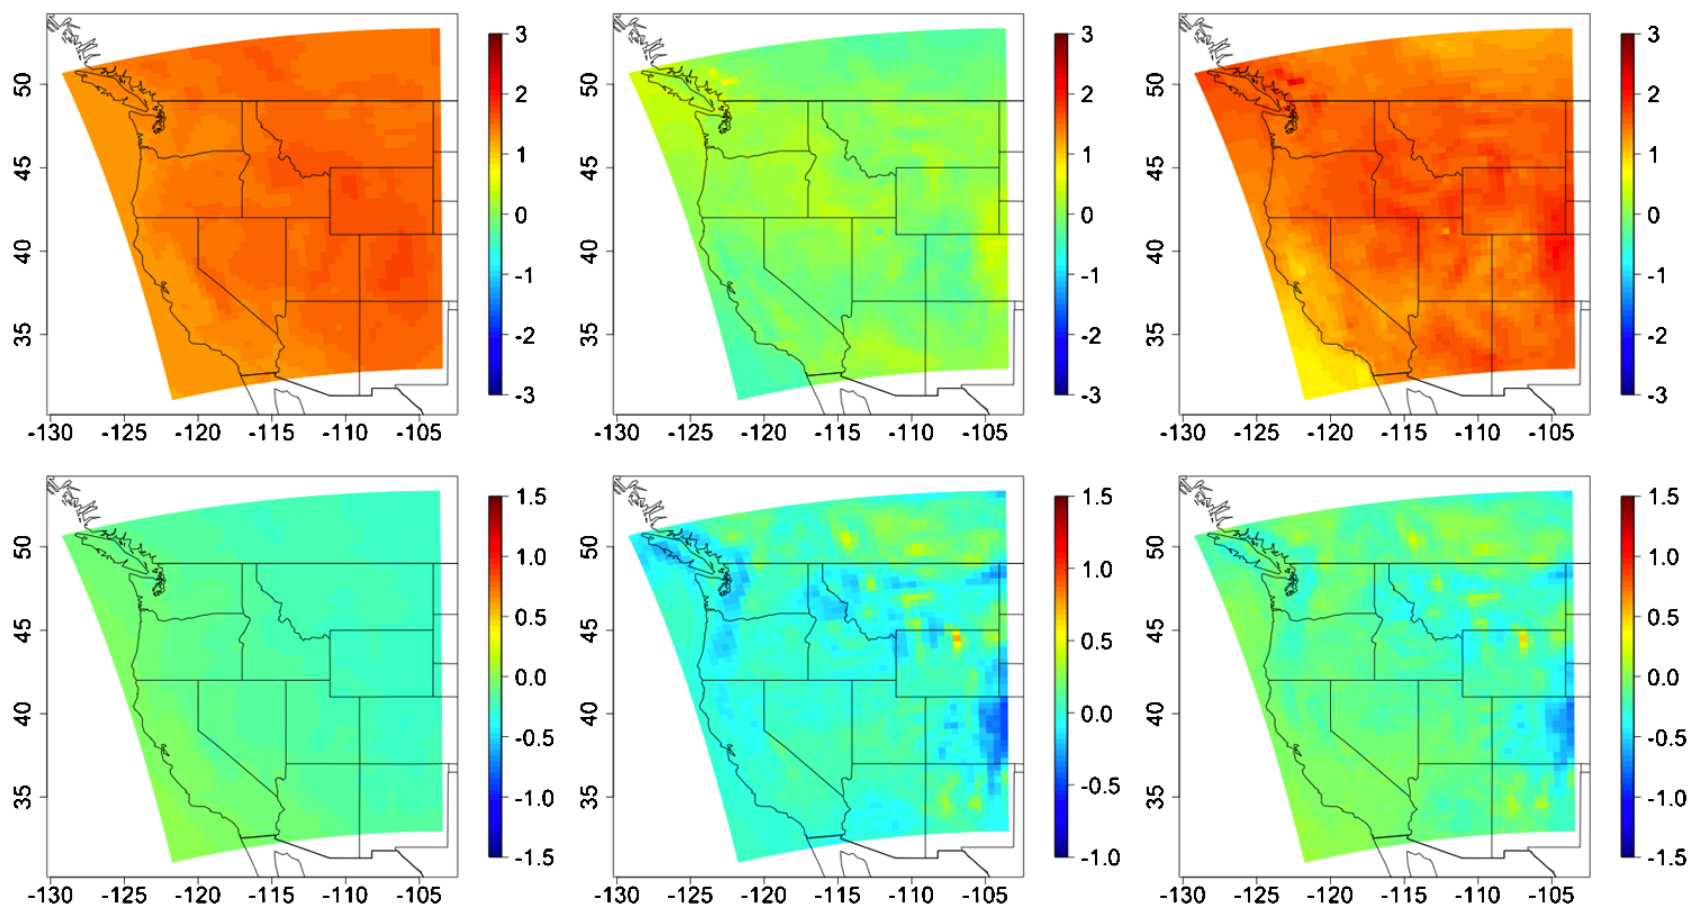
\includegraphics[width = 0.8\textwidth]{Fig10.png}
    \caption{\emph{Posterior means for the regression (left), the spatial effect (middle), and the sum (right) for the summer season. The top row represents the change in midpoint temperature ($^\circ K$), while the bottom represents the change in total precipitation (inches).}}
    \label{fig: Fig10}
\end{figure}

A hierarchical clustering was performed and summarized in Figure \ref{fig: Fig11}. There appears to be more widespread warming and decreasing total precipitation during the summer months. 

\begin{figure}[H]
    \centering
    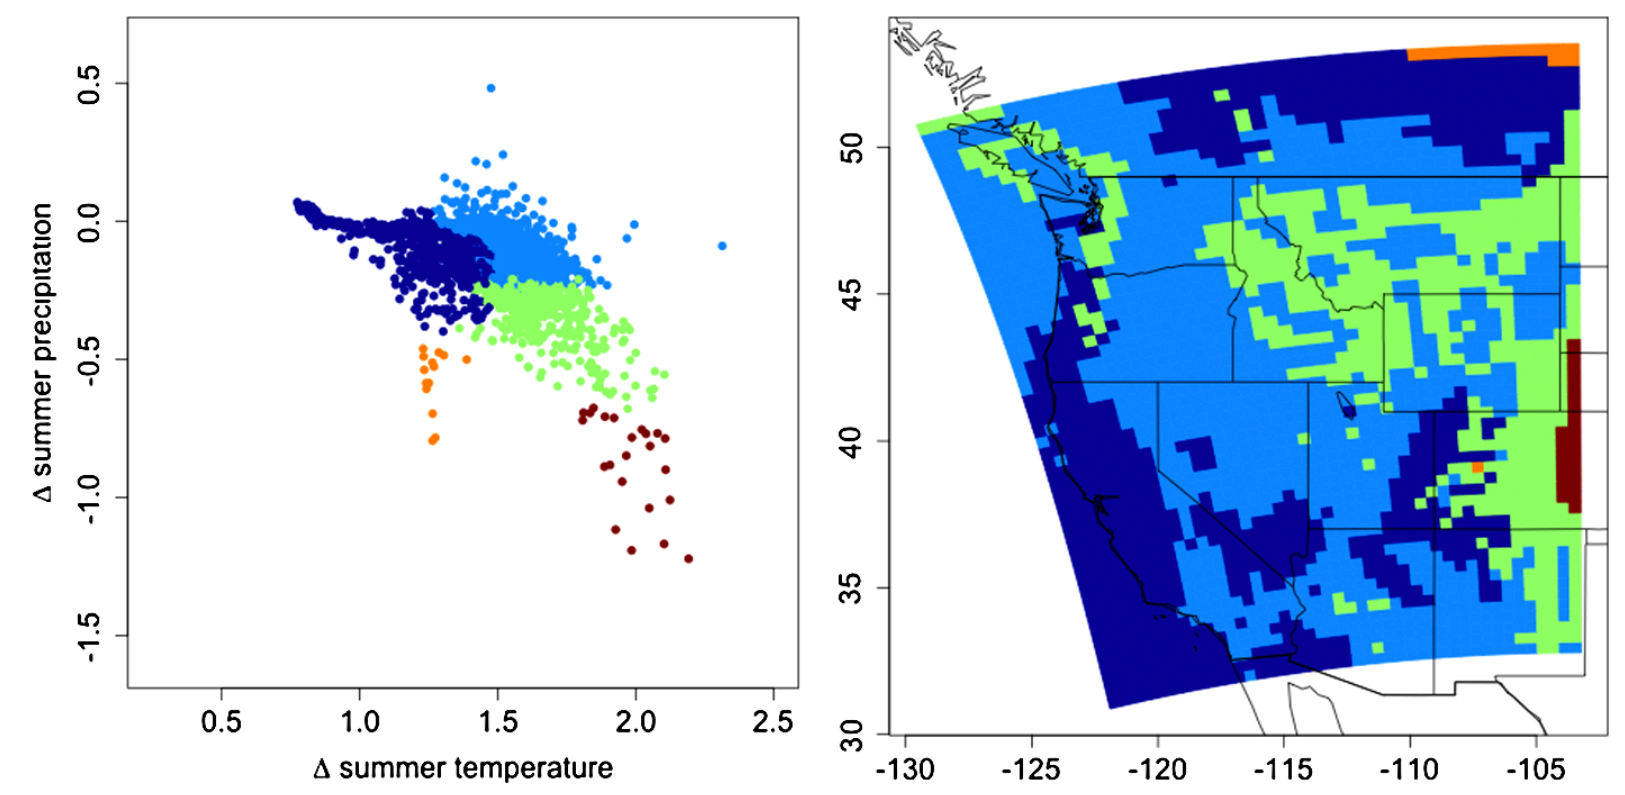
\includegraphics[width = 0.8\textwidth]{Fig11.png}
    \caption{\emph{Results from clustering the posterior means of the change in temperature and total precipitation for the summer season. The left frame is a scatterplot with the clusters indicated through different colors. The right frame shows the clusters spatially.}}
    \label{fig: Fig11}
\end{figure}

Figure \ref{fig: Fig12} shows estimated pointwise probabilities. In general, summer warming and decreasing total precipitation is widespread, even more so than in the winter season, and focused more on the eastern side of the domain.

\begin{figure}[H]
    \centering
    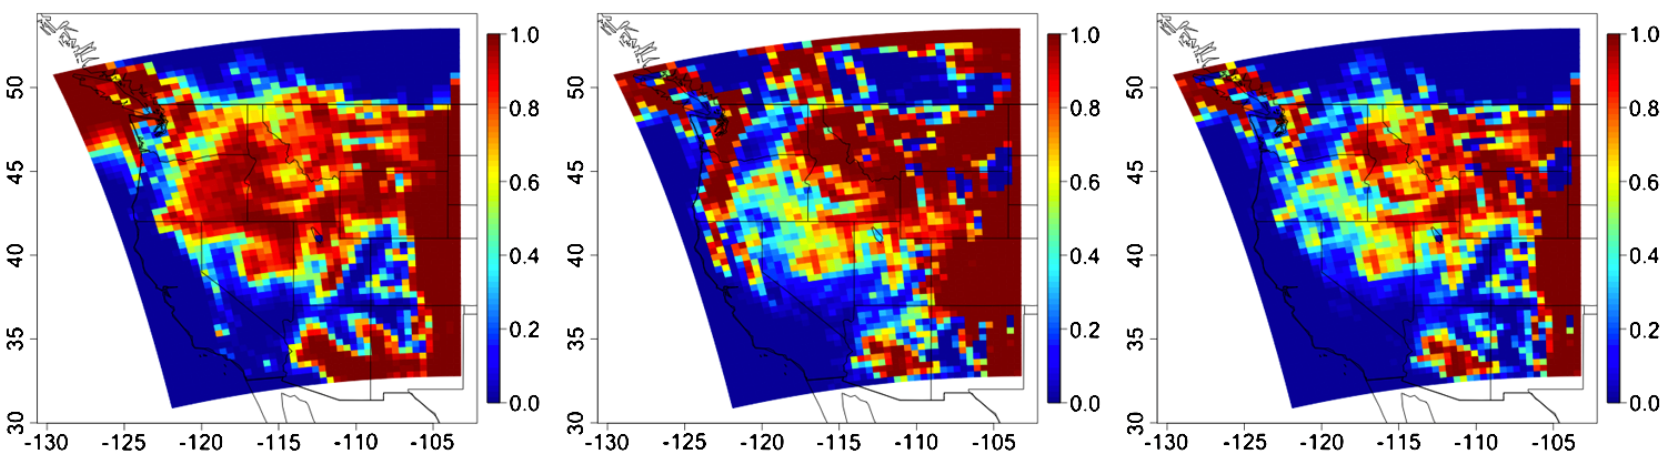
\includegraphics[width = 0.8\textwidth]{Fig12.png}
    \caption{\emph{Estimated pointwise probabilities for the summer season: increasing temperature (left), decreasing total precipitation (middle), and simultaneously increasing temperature and decreasing total precipitation (right).}}
    \label{fig: Fig12}
\end{figure}

Figure \ref{fig: Fig13} is constructed similarly to Figure \ref{fig: Fig8}. However, the stronger negative correlation in the summer season is more apparent in the figure. The large decreases in total precipitation are strongest in the eastern portion of the domain, but decrease dramatically when we condition on larger increases in temperature.

\begin{figure}[H]
    \centering
    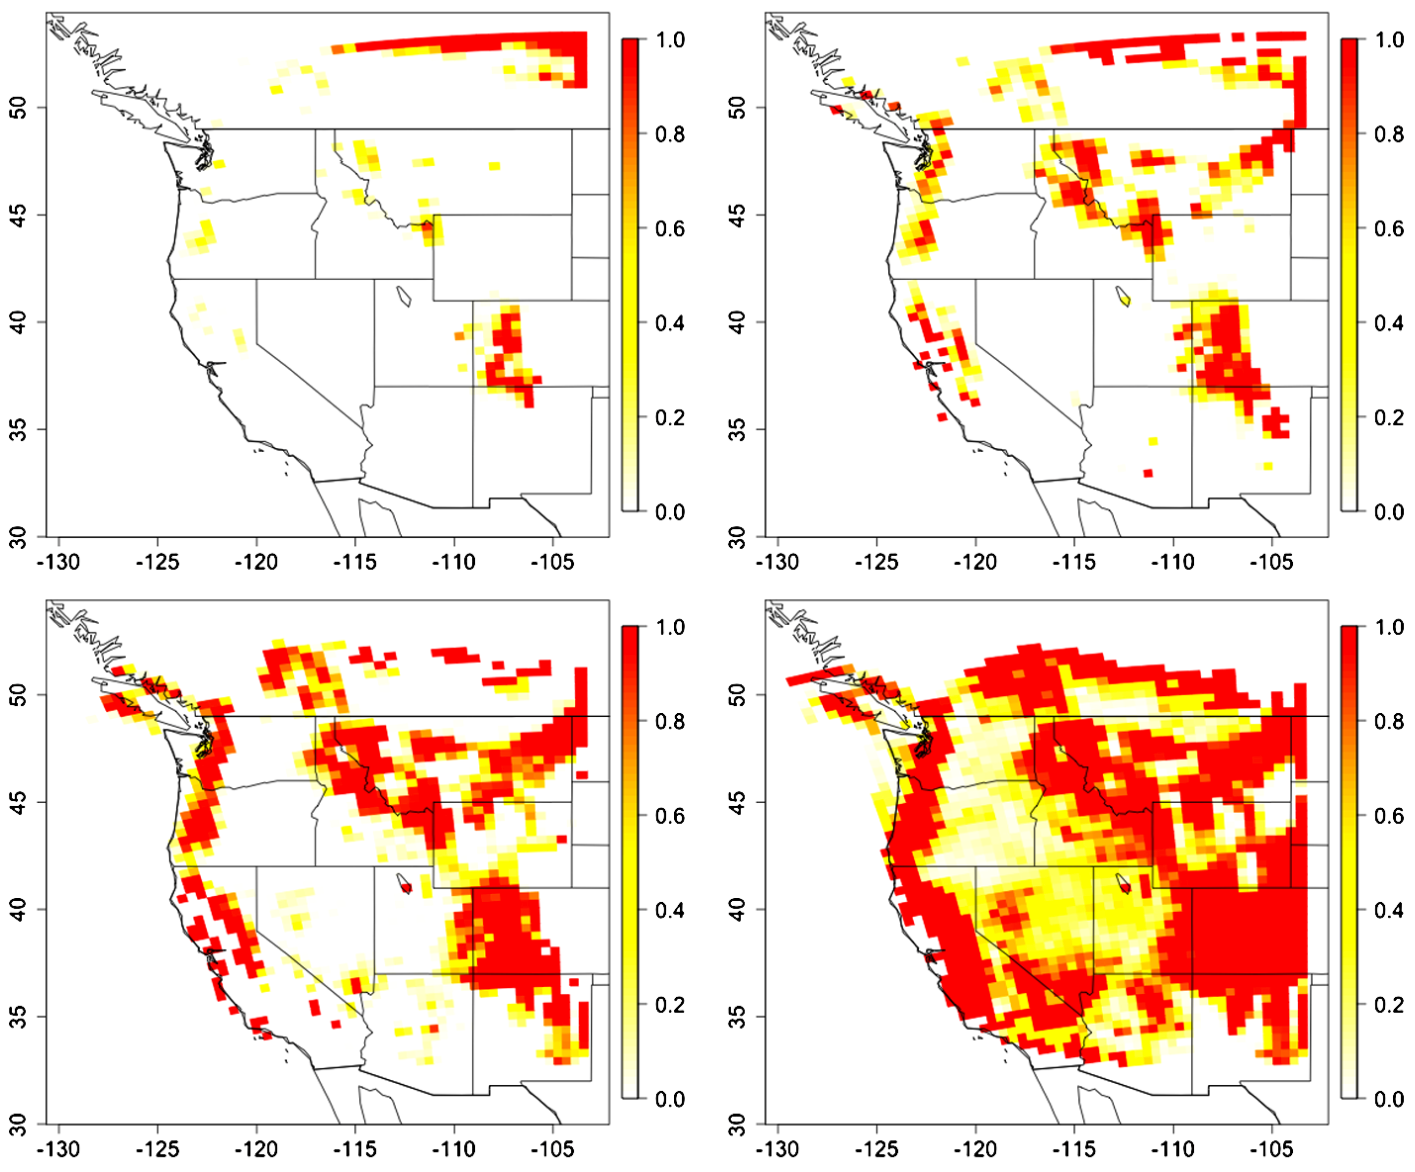
\includegraphics[width = 0.8\textwidth]{Fig13.png}
    \caption{\emph{Probability of a large decrease in summer total precipitation, conditional on the increase in temperature falling in the first quartile (top left), second quartile (top right), third quartile (bottom left), and fourth quartile (bottom right).}}
    \label{fig: Fig13}
\end{figure}

The contours in Figure \ref{fig: Fig14} suggest larger increases in temperature and decreases in total precipitation (on average) for the Denver area, while the contour for the Sacramento area suggests more modest changes on both variables.

\begin{figure}[H]
    \centering
    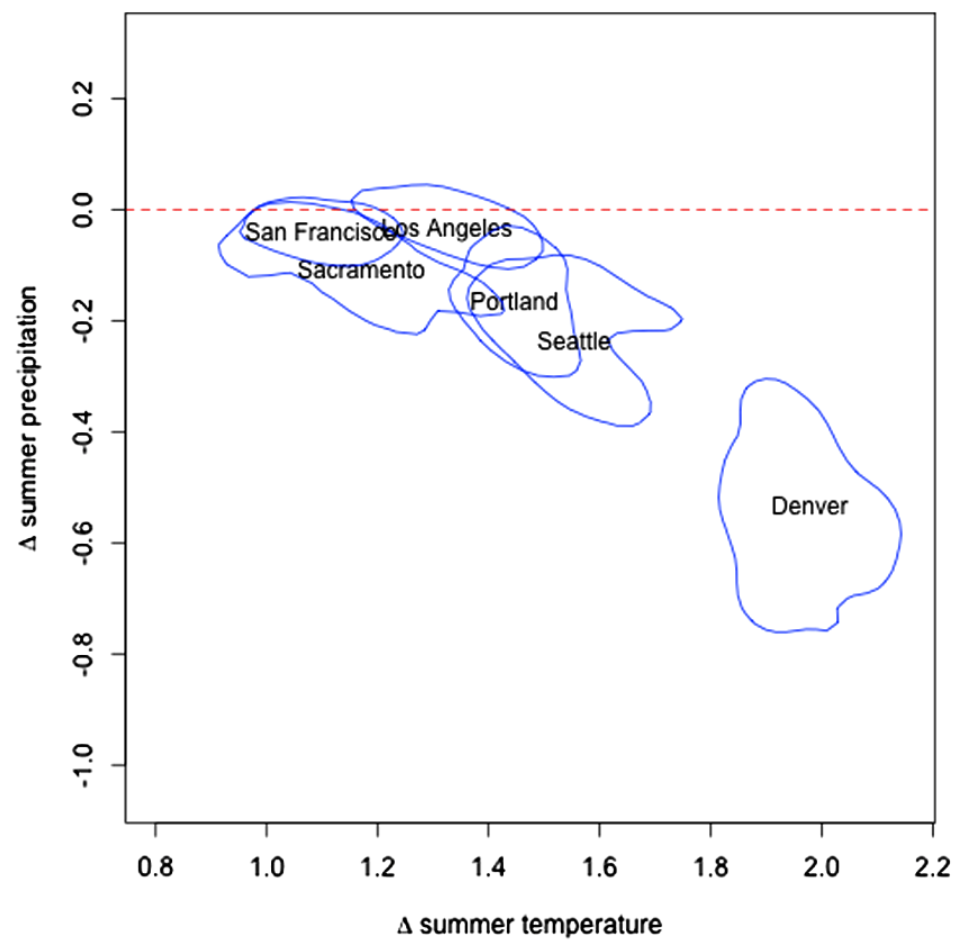
\includegraphics[width = 0.8\textwidth]{Fig14.png}
    \caption{\emph{Approximate 95\% contours for the average change in summer temperature and precipitation for the grid boxes associated with the five consolidated metropolitan statistical areas in the domain.}}
    \label{fig: Fig14}
\end{figure}

\bibliographystyle{apalike} 
\bibliography{References.bib} 

\end{document}
